\documentclass{sigchi}

% Use this section to set the ACM copyright statement (e.g. for
% preprints).  Consult the conference website for the camera-ready
% copyright statement.

% Copyright
\CopyrightYear{2020}
%\setcopyright{acmcopyright}
\setcopyright{acmlicensed}
%\setcopyright{rightsretained}
%\setcopyright{usgov}
%\setcopyright{usgovmixed}
%\setcopyright{cagov}
%\setcopyright{cagovmixed}
% DOI
\doi{https://doi.org/10.1145/3313831.XXXXXXX}
% ISBN
\isbn{978-1-4503-6708-0/20/04}
%Conference
\conferenceinfo{CHI'20,}{April  25--30, 2020, Honolulu, HI, USA}
%Price
\acmPrice{\$15.00}

% Use this command to override the default ACM copyright statement
% (e.g. for preprints).  Consult the conference website for the
% camera-ready copyright statement.

%% HOW TO OVERRIDE THE DEFAULT COPYRIGHT STRIP --
%% Please note you need to make sure the copy for your specific
%% license is used here!
% \toappear{
% Permission to make digital or hard copies of all or part of this work
% for personal or classroom use is granted without fee provided that
% copies are not made or distributed for profit or commercial advantage
% and that copies bear this notice and the full citation on the first
% page. Copyrights for components of this work owned by others than ACM
% must be honored. Abstracting with credit is permitted. To copy
% otherwise, or republish, to post on servers or to redistribute to
% lists, requires prior specific permission and/or a fee. Request
% permissions from \href{mailto:Permissions@acm.org}{Permissions@acm.org}. \\
% \emph{CHI '16},  May 07--12, 2016, San Jose, CA, USA \\
% ACM xxx-x-xxxx-xxxx-x/xx/xx\ldots \$15.00 \\
% DOI: \url{http://dx.doi.org/xx.xxxx/xxxxxxx.xxxxxxx}
% }

% Arabic page numbers for submission.  Remove this line to eliminate
% page numbers for the camera ready copy
% \pagenumbering{arabic}

% Load basic packages
\usepackage{balance}       % to better equalize the last page
\usepackage{graphics}      % for EPS, load graphicx instead 
\usepackage[T1]{fontenc}   % for umlauts and other diaeresis
\usepackage{txfonts}
\usepackage{mathptmx}
\usepackage[pdflang={en-US},pdftex]{hyperref}
\usepackage{color}
\usepackage{booktabs}
\usepackage{textcomp}

% Some optional stuff you might like/need.
\usepackage{microtype}        % Improved Tracking and Kerning
% \usepackage[all]{hypcap}    % Fixes bug in hyperref caption linking
\usepackage{ccicons}          % Cite your images correctly!
% \usepackage[utf8]{inputenc} % for a UTF8 editor only

% If you want to use todo notes, marginpars etc. during creation of
% your draft document, you have to enable the "chi_draft" option for
% the document class. To do this, change the very first line to:
% "\documentclass[chi_draft]{sigchi}". You can then place todo notes
% by using the "\todo{...}"  command. Make sure to disable the draft
% option again before submitting your final document.
\usepackage{todonotes}

% Paper metadata (use plain text, for PDF inclusion and later
% re-using, if desired).  Use \emtpyauthor when submitting for review
% so you remain anonymous.
\def\plaintitle{Space Folding in Virtual Reality}
\def\plainauthor{Joe Strout}
\def\emptyauthor{}
\def\plainkeywords{virtual reality;travel;nonphysical spaces}
\def\plaingeneralterms{Virtual Reality}

% llt: Define a global style for URLs, rather that the default one
\makeatletter
\def\url@leostyle{%
  \@ifundefined{selectfont}{
    \def\UrlFont{\sf}
  }{
    \def\UrlFont{\small\bf\ttfamily}
  }}
\makeatother
\urlstyle{leo}

% To make various LaTeX processors do the right thing with page size.
\def\pprw{8.5in}
\def\pprh{11in}
\special{papersize=\pprw,\pprh}
\setlength{\paperwidth}{\pprw}
\setlength{\paperheight}{\pprh}
\setlength{\pdfpagewidth}{\pprw}
\setlength{\pdfpageheight}{\pprh}

% Make sure hyperref comes last of your loaded packages, to give it a
% fighting chance of not being over-written, since its job is to
% redefine many LaTeX commands.
\definecolor{linkColor}{RGB}{6,125,233}
\hypersetup{%
  pdftitle={\plaintitle},
% Use \plainauthor for final version.
%  pdfauthor={\plainauthor},
  pdfauthor={\emptyauthor},
  pdfkeywords={\plainkeywords},
  pdfdisplaydoctitle=true, % For Accessibility
  bookmarksnumbered,
  pdfstartview={FitH},
  colorlinks,
  citecolor=black,
  filecolor=black,
  linkcolor=black,
  urlcolor=linkColor,
  breaklinks=true,
  hypertexnames=false
}

% create a shortcut to typeset table headings
% \newcommand\tabhead[1]{\small\textbf{#1}}

% End of preamble. Here it comes the document.
\begin{document}

\title{\plaintitle}

\numberofauthors{1}
\author{%
  \alignauthor{Joe Strout\\
    \affaddr{Colorado State University}\\
    \affaddr{Fort Collins, United States}\\
    \email{joe@strout.net}}\\
}

\maketitle

\begin{abstract}
  UPDATED---\today. Abstract here will describe the VR space folding technique, summarizing background, methods, results, and conclusion.  Aim for about 150 words.
\end{abstract}


% ACM Classfication

\begin{CCSXML}
<ccs2012>
<concept>
<concept_id>10003120.10003121</concept_id>
<concept_desc>Human-centered computing~Human computer interaction (HCI)</concept_desc>
<concept_significance>500</concept_significance>
</concept>
<concept>
<concept_id>10003120.10003121.10003125.10011752</concept_id>
<concept_desc>Human-centered computing~Haptic devices</concept_desc>
<concept_significance>300</concept_significance>
</concept>
<concept>
<concept_id>10003120.10003121.10003122.10003334</concept_id>
<concept_desc>Human-centered computing~User studies</concept_desc>
<concept_significance>100</concept_significance>
</concept>
</ccs2012>
\end{CCSXML}

\ccsdesc[500]{Human-centered computing~Human computer interaction (HCI)}
\ccsdesc[300]{Human-centered computing~Haptic devices}
\ccsdesc[100]{Human-centered computing~User studies}

% Author Keywords
\keywords{\plainkeywords}

% Print the classficiation codes
\printccsdesc
Please use the 2012 Classifiers and see this link to embed them in the text: \url{https://dl.acm.org/ccs/ccs_flat.cfm}



\section{Introduction}

Real walking is widely regarded as the most natural and direct travel technique.  It provides vestibular cues, requires no training, promotes spatial understanding, and is especially efficient at maneuvering tasks.  However, it is not widely adopted in consumer VR applications primarily because of the limits of the user's physical area.  Current consumer headsets are designed for indoor use only, and most users do not have an indoor space larger than a few meters on a side.

While many approaches have been developed to "compress" a larger virtual space into a smaller physical one (see Related Work), various limitations make these difficult to apply to a room-scale VR setup of say 3 by 4 meters area, or limit the amount of extra space gained to a modest factor of less than 2X.

Here we introduce an approach to spatial compression that allows for any compression factor, works in a space as small as 2 by 3 meters, and works with completely natural walking, without redirection.  Of course there are always trade-offs; the technique presented works best for indoor virtual scenes, and makes no attempt to keep the user from noticing the spatial manipulation.  We present an experiment to show that this does not detract from the user's ability to navigated the virtual environment, or in overall user satisfaction.


\begin{figure*}[htb]
  \centering
  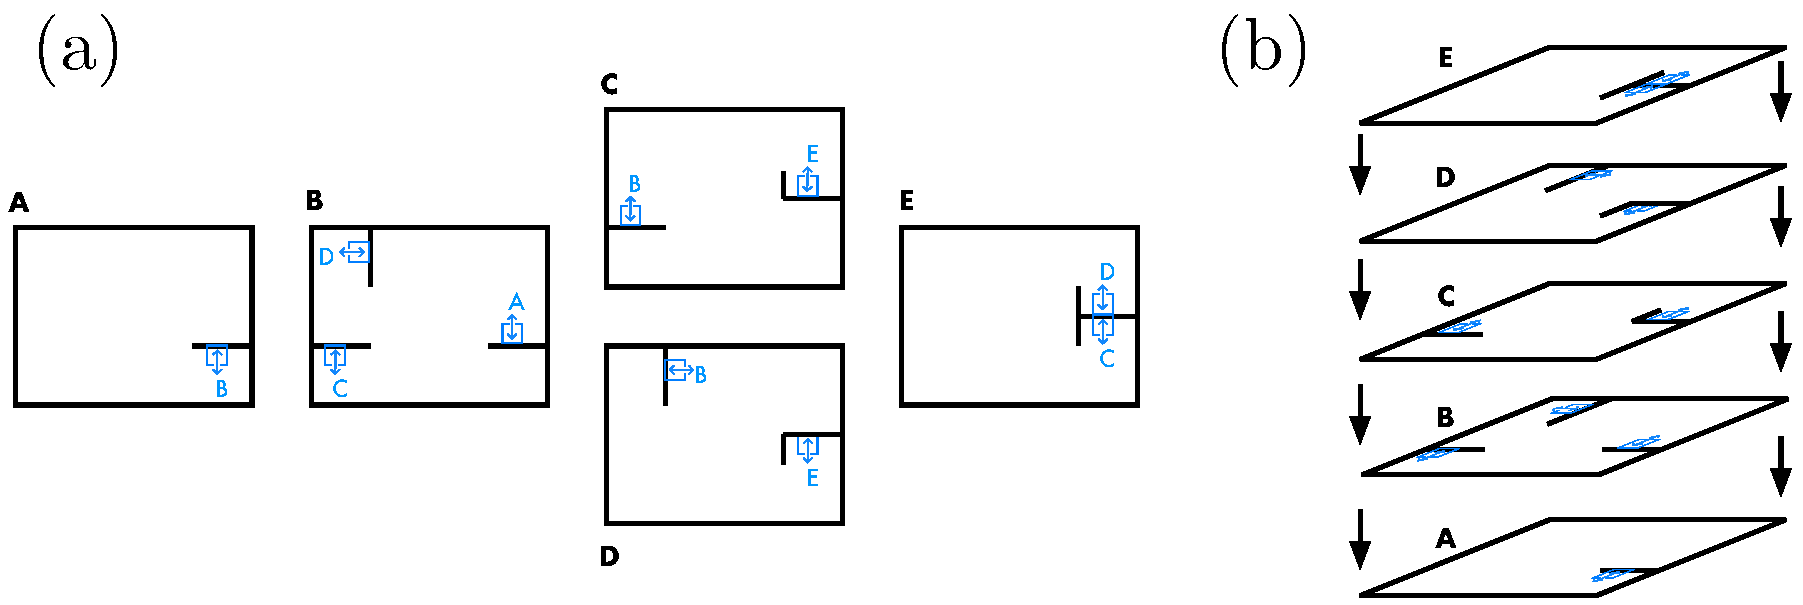
\includegraphics[width=1.75\columnwidth]{figures/FoldingDiagram.pdf}
  \caption{Illustration of the space folding technique.  Each "room" of the virtual environment contains portals that connect to other rooms, allowing both viewing and travel in both directions.  The layout shown here was used in the pilot study.  In (a) the five rooms are shown in top-down view, separated for clarity; (b) illustrates how these virtual spaces are "folded" into one physical space.}~\label{fig:foldingDiagram}
\end{figure*}


\section{Related Work}

Here we review previous work.  This could be part of the Introduction section, or it could be a separate section as we have it here.

Vaslevska \& Kaufman~\cite{vasylevska2017compressing} reviewed several techniques for compressing virtual environments to enable natural locomotion within a limited physical space.  

Field and Vamplew~\cite{field2004generalised} extended earlier redirected walking work with additional algorithms to redirect the user to the center of the physical space, and to keep the user on circular paths that anticipate possible future turns.  (No actual VR experiments were used in testing this system.)

Experiments comparing four redirected walking algorithms were carried out by Hodgson and Bachmann~\cite{hodgson2013comparing}.  Subjects walked within a 25m x 45m facility under either normal conditions, or while using redirection.  The authors also did simulations of agents moving at 1m/s, considered typical of VR users.  Their experiments determined that a 35m x 35m space would be needed for such locomotion in an unconstrained virtual environment.

Nilsson et al reviewed 15 years of redirected walking research, summarizing the state of the field in 2018~\cite{nilsson201815}.

A very different approach to compressing a virtual environment is change blindness redirection, explored by Suma et al~\cite{suma2011leveraging}.  With this technique, the layout of some part of the VE is changed when the user isn't looking at it.  For example, a doorway may be moved from one wall to another while the user is looking away or their view is occluded.  The technique produces a powerful illusion of a large VE, but requires the user to follow particular paths; it does not allow for free exploration.

Suma and Krum introduced the term \textit{impossible spaces} to describe a closely related technique, in which rooms are spatially expanded while not in view, thus producing a self-overlapping architecture~\cite{suma2012impossible}.  The authors were intent on maintaining the illusion of a natural space, and found that rooms could overlap by as much as 56\% before users began to notice.  The present work could be considered an extreme version of impossible spaces, in which the objective to keep users from noticing is abandoned, and a much higher overlap factor is obtained.

While many spatial compression studies focus on measuring the ability of users to detect the manipulation, Peck et al~\cite{peck2011evaluation} instead compared several measures of navigability for redirected walking (with distractors to create redirection opportunities), walking-in-place, and joystick locomotion.  (In the latter case, travel speed was proportional to joystick deflection, with a top speed of 3 mph.)


\section{Methods}

\subsection{Technique}

An illustration of the VR Space Folding technique is shown in Figure ~\ref{fig:foldingDiagram}.  The central idea is relatively simple: the virtual environment (VE) is divided into spaces ("rooms"), joined by portals.  Stepping through a portal takes the user to a different virtual space, which occupies the same physical space as the previous room.  In this way, an arbitrarily large VE can be "folded" into a restricted physical environment.

While the core idea would work with opaque portals, the experience is enhanced by portals that can be seen through.  For example, when standing in the southeast corner of the physical space while in room $A$ of Figure~\ref{fig:foldingDiagram} (assuming north is towards the top of the diagram), and looking north, one would see part of room $B$, just as if looking through an ordinary arch or open doorway.  Stepping through that doorway, and then turning around and looking south, one would see the corner of room $A$ just vacated.

The technique places two important constraints on the placement of the connecting portals:

1. Because the user must be able to physically walk through them, portals may not be placed on the outside boundary of the physical space.  Instead they must turned perpendicular to that boundary, or otherwise moved away from the outside edge so that the user has room to walk on both sides of each portal.

2. Each portal has a specific location in physical space, which must be the same as its position in \textit{both} virtual spaces it connects.  We cannot, for example, connect the west side of one room to the east side of another.

However, within these constraints, portal placement is otherwise free.  In this pilot study we have placed all portals orthogonal to the room walls, but that is not necessary.  Within a single virtual room, a portal is one-sided, as in the aforementioned portal between rooms A and B; this is traversed only northward from room A, or southward from room B.  But two portals may be placed back-to-back, as illustrated by the portals from room E to rooms C and D.  In this example, looking through the archway from the south one would see room C; but looking through it from the north, one would see room D.

The set of connected virtual rooms form an undirected, connected graph.  The graph size is the number of rooms, and its order is equal to the largest number of portals in any room.  In most applications this order is likely to be relatively low, as each portal takes up roughly $2 m^2$ of physical space.  We can therefore enumerate the possible room graphs.  An order 1 graph (i.e. no more than one portal per room) is always exactly two rooms.  There are two possible order 2 (two portals per room) graphs, regardless of size: either all rooms connected in a line, or the end rooms also joined to form a loop.

\begin{figure*}[htb]
  \centering
  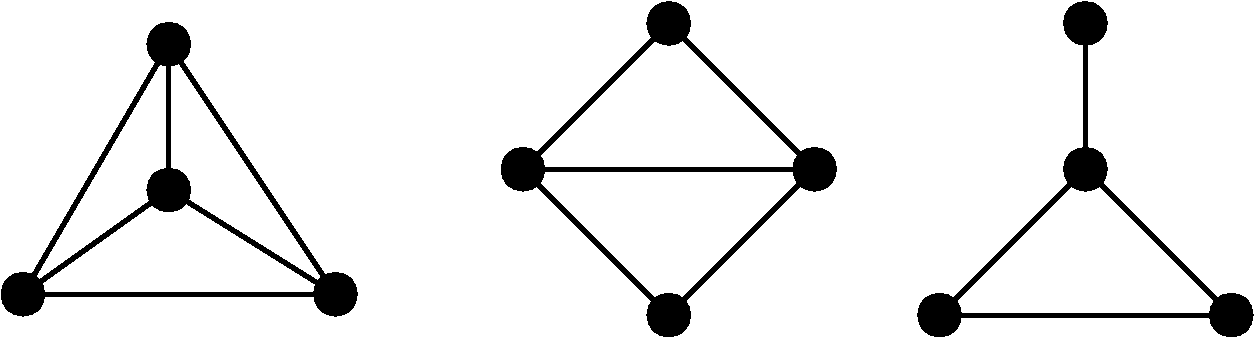
\includegraphics[width=1\columnwidth]{figures/Size4Graphs.pdf}
  \caption{All possible order-3 graphs of 4 nodes.  These are the possible topologies for a VE with 4 rooms and up to 3 doors per room.}~\label{fig:size4Graphs}
\end{figure*}

\begin{figure*}[htb]
  \centering
  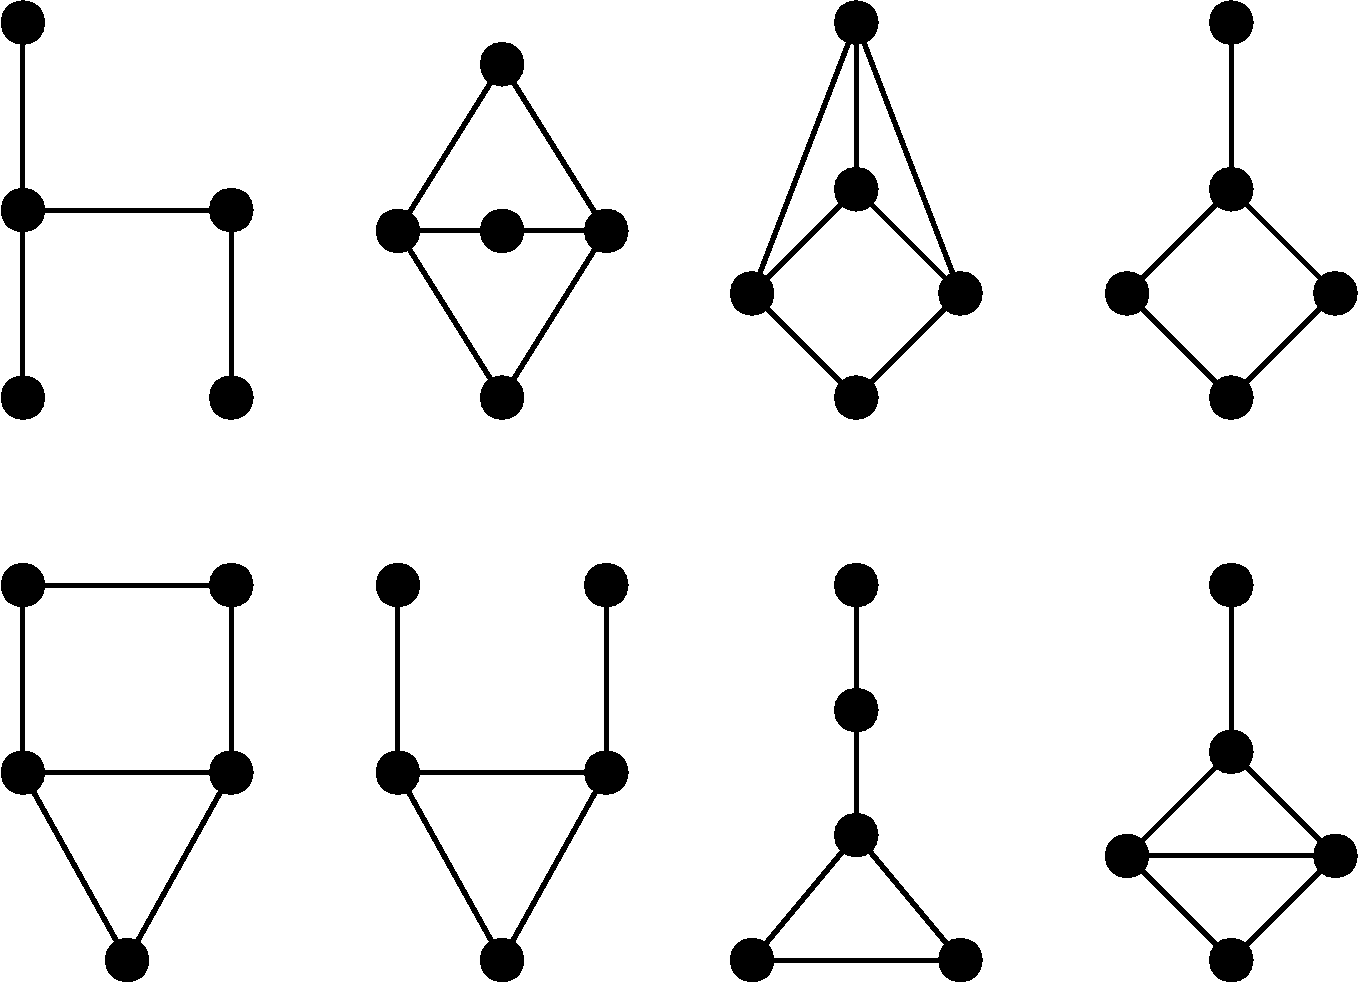
\includegraphics[width=1\columnwidth]{figures/Size5Graphs.pdf}
  \caption{All possible order-3 graphs of 5 nodes.  The room layout shown in Figure~\ref{fig:foldingDiagram} and used in the pilot study corresponds to the top-right graph above.}~\label{fig:size5Graphs}
\end{figure*}

Once we allow order 3 (up to three portals per room), the design possibilities expand considerably.  The smallest order-3 graph has four nodes, and there are exactly three such graphs, shown in Figure~\ref{fig:size4Graphs}.  Any arrangement of four rooms, with no more than three portals per room, will be isomorphic to one of these.  Similarly, with five rooms, the layout will be isomorphic to one of the eight graphs shown in Figure~\ref{fig:size5Graphs}.  Larger or higher-order graphs are of course possible too.  While there is in principle no limit to the size or order of the graph layout one could use, order 3 is the smallest order which allows a wide variety of possible designs, and will be taken as a minimal requirement when considering implementation details.

\subsection{Implementation Details}

- Portal code requirements.

- Shader approach.

\subsection{Pilot Study}

\section{Results}

\section{Discussion}

- Limitations of shader approach used.

- Other technical limitations.

- Limitations of the pilot study.

- Implications for VE design; when this approach is (and is not) appropriate.
	- needs at least 3 x 2 meters
	- works best for indoor environments
	- very large VE's might get tedious, but
	- shortcuts (normal portals, plus teleporters/elevators) are possible

\section{Conclusion}

- Summary of approach.

- Summary of findings.

- Possible directions for future work.

\section{Acknowledgments}

Here thanking everybody who helped out.

% Balancing columns in a ref list is a bit of a pain because you
% either use a hack like flushend or balance, or manually insert
% a column break.  http://www.tex.ac.uk/cgi-bin/texfaq2html?label=balance
% multicols doesn't work because we're already in two-column mode,
% and flushend isn't awesome, so I choose balance.  See this
% for more info: http://cs.brown.edu/system/software/latex/doc/balance.pdf
%
% Note that in a perfect world balance wants to be in the first
% column of the last page.
%
% If balance doesn't work for you, you can remove that and
% hard-code a column break into the bbl file right before you
% submit:
%
% http://stackoverflow.com/questions/2149854/how-to-manually-equalize-columns-
% in-an-ieee-paper-if-using-bibtex
%
% Or, just remove \balance and give up on balancing the last page.
%
\balance{}

% REFERENCES FORMAT
% References must be the same font size as other body text.
\bibliographystyle{SIGCHI-Reference-Format}
\bibliography{sample}

\end{document}

%%% Local Variables:
%%% mode: latex
%%% TeX-master: t
%%% End:
